\documentclass[11pt,a4paper]{article}
\usepackage[top=16mm,bottom=17mm,left=16mm,right=16mm,headheight=0pt,headsep=0mm,footskip=10mm]{geometry}
\usepackage{iftex}
\ifPDFTeX
 \usepackage[utf8]{inputenc}
 \usepackage[T5]{fontenc}
 \usepackage{mathptmx}
\else
 \usepackage{mathptmx}
 \usepackage{fontspec}
 \IfFontExistsTF{Times New Roman}{\setmainfont{Times New Roman}}{\IfFontExistsTF{TeXGyreTermes}{\setmainfont{TeXGyreTermes}}{\setmainfont{Latin Modern Roman}}}
\fi
\usepackage{amsmath,amssymb}
\usepackage{xcolor,tikz,enumitem,multicol,fancyhdr,lastpage}
\usepackage[most]{tcolorbox}
% Giu phong cach, mau sac va bo cuc cua Toan_11_04.tex.
\definecolor{questionpurple}{RGB}{137,38,143}
\definecolor{answerblue}{RGB}{35,45,140}
\definecolor{lightblue}{RGB}{238,245,255}
\setlength{\parindent}{0pt}
\setlength{\parskip}{0pt}
\renewcommand{\baselinestretch}{1.10}
\setlength{\columnsep}{8mm}
\pagestyle{fancy}
\fancyhf{}
\renewcommand{\headrulewidth}{0pt}
\fancyfoot[L]{\small Chuyên đề III -- Toán 11}
\fancyfoot[R]{\small Trang \thepage/\pageref{LastPage} -- Bài 07}
\renewcommand{\footrulewidth}{.4pt}
\setlist[itemize]{leftmargin=6mm,label=\textcolor{answerblue}{\textbullet},itemsep=2pt,topsep=3pt,parsep=0pt}
\setlist[enumerate]{leftmargin=8mm,itemsep=4pt,topsep=3pt,parsep=0pt}
\newtcolorbox{theorybox}{colback=lightblue,colframe=answerblue!60,boxrule=.5pt,
 arc=1mm,left=2.5mm,right=2.5mm,top=1.5mm,bottom=1.5mm,before skip=3pt,after skip=4pt}
\newcommand{\sectitle}[2]{\vspace{4pt}\noindent{\large\bfseries\textcolor{questionpurple}{#1.\ #2}}\par\vspace{3pt}}
\newcommand{\exampletitle}[2]{\vspace{3pt}\noindent{\bfseries\textcolor{answerblue}{Ví dụ #1.}} #2\par\vspace{2pt}}
\newcommand{\compactproblems}{\setlist[enumerate,1]{label=\textcolor{questionpurple}{\bfseries\arabic*.},leftmargin=7mm,labelsep=1.5mm,itemsep=3pt,topsep=2pt}}
\newcommand{\sinegraph}{%
 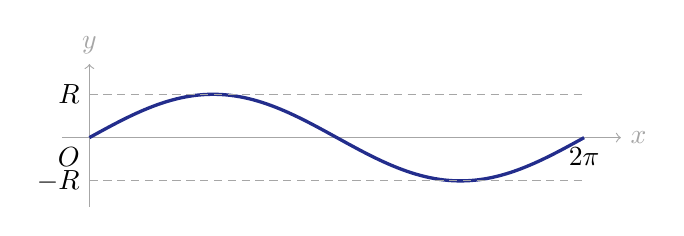
\begin{tikzpicture}[x=1.0cm,y=.55cm,baseline=(current bounding box.center)]
   \draw[->,gray!70] (-.35,0)--(6.75,0) node[right] {$x$};
   \draw[->,gray!70] (0,-1.6)--(0,1.7) node[above] {$y$};
   \draw[answerblue,very thick,domain=0:6.283,samples=110] plot (\x,{sin(\x r)});
   \draw[densely dashed,gray!70] (0,1)--(6.3,1) (0,-1)--(6.3,-1);
   \node[left] at (0,1) {$R$}; \node[left] at (0,-1) {$-R$};
   \node[below left] at (0,0) {$O$};
   \node[below] at (6.283,0) {$2\pi$};
 \end{tikzpicture}}


% Bo sung khoang cach gon, phu hop ban de khong co khoang trong de giai.
\setlength{\abovedisplayskip}{5pt}
\setlength{\belowdisplayskip}{5pt}
\setlength{\abovedisplayshortskip}{3pt}
\setlength{\belowdisplayshortskip}{3pt}
\setlist[enumerate]{leftmargin=8mm,itemsep=2pt,topsep=2pt,parsep=0pt}
\raggedbottom
\newcommand{\propertytitle}[1]{\par\vspace{3pt}\noindent\textbf{\textcolor{answerblue}{#1}}\enspace}
\newcommand{\mplane}[1]{\left(#1\right)}
\newcommand{\srcnote}[1]{{\footnotesize\textcolor{black!70}{#1}}}
\newcommand{\drawpoint}[3]{\fill[answerblue] (#1) circle (1.4pt) node[#2] {$#3$};}

\begin{document}
\noindent
\begin{minipage}[t]{.35\linewidth}
 \centering{\bfseries CHUYÊN ĐỀ III -- TOÁN -- 11\par}
 \vspace{2pt}\rule{.73\linewidth}{.4pt}\par\vspace{3pt}
 CHỦ ĐỀ 03\par\vspace{3pt}{\itshape TÀI LIỆU HỌC TẬP -- BÀI 07\par}
\end{minipage}\hfill
\begin{minipage}[t]{.62\linewidth}
 \centering{\bfseries HÌNH HỌC KHÔNG GIAN\par}
 \vspace{4pt}{\small\bfseries VẤN ĐỀ 11X31\par
 CƠ BẢN VỀ HÌNH HỌC KHÔNG GIAN\par}
\end{minipage}

\vspace{4mm}
\noindent\textbf{Họ và tên:}\dotfill\hfill\textbf{Lớp:}\enspace\dotfill
\vspace{2mm}

\begin{theorybox}
\textbf{Kiến thức trọng tâm:} Mặt phẳng và quan hệ thuộc; sáu tính chất thừa nhận;
ba cách xác định mặt phẳng; hình chóp, hình tứ diện; phương pháp xác định
giao tuyến của hai mặt phẳng và giao điểm của đường thẳng với mặt phẳng.
\end{theorybox}

\sectitle{1}{Khái niệm mở đầu}
\begin{itemize}
 \item Mặt bảng, màn hình máy tính, mặt nước hồ yên lặng là hình ảnh về
 một phần của \textbf{mặt phẳng}. Mặt phẳng không có bề dày và không có giới hạn.
 \item Mặt phẳng thường được kí hiệu bằng chữ cái in hoa hoặc chữ cái Hy Lạp
 trong ngoặc: $(P)$, $(Q)$, $(\alpha)$, $(\beta)$.
 \item Để biểu diễn mặt phẳng, ta vẽ hình bình hành hoặc một miền góc,
 rồi ghi tên mặt phẳng tại một góc.
 \item Nếu điểm $A$ thuộc mặt phẳng $(\alpha)$, viết
 $\boxed{A\in(\alpha)}$. Nếu điểm $B$ không thuộc $(\alpha)$, viết
 $\boxed{B\notin(\alpha)}$.
\end{itemize}

\begin{center}
\begin{tikzpicture}[scale=.76,>=stealth]
  \fill[lightblue] (0,0)--(2.9,0)--(3.7,1.12)--(.8,1.12)--cycle;
  \draw[answerblue,thick] (0,0)--(2.9,0)--(3.7,1.12)--(.8,1.12)--cycle;
  \node[answerblue] at (.52,.24) {$(\alpha)$};
  \drawpoint{2.15,.58}{above}{A}
  \drawpoint{3.65,1.6}{right}{B}
  \node[below] at (1.85,-.27) {\small $A\in(\alpha),\quad B\notin(\alpha)$};
  \begin{scope}[xshift=6.2cm]
    \fill[lightblue] (0,0)--(2.25,0)--(2.85,.9)--(.6,.9)--cycle;
    \draw[answerblue,thick] (0,0)--(2.25,0)--(2.85,.9)--(.6,.9)--cycle;
    \node[answerblue] at (.5,.24) {$P$};
    \node[below] at (1.4,-.27) {\small Hình biểu diễn mặt phẳng};
  \end{scope}
\end{tikzpicture}
\end{center}

\textbf{Quy tắc biểu diễn hình không gian:}
\begin{itemize}
 \item Đường thẳng, đoạn thẳng được biểu diễn tương ứng bằng đường thẳng, đoạn thẳng.
 \item Hai đường thẳng song song hoặc cắt nhau được biểu diễn bằng hai đường thẳng
 song song hoặc cắt nhau.
 \item Giữ nguyên quan hệ thuộc giữa điểm và đường thẳng.
 \item Nét liền biểu diễn đường nhìn thấy; nét đứt biểu diễn đường bị che khuất.
\end{itemize}
\begin{center}
\begin{tikzpicture}[scale=.78,line join=round]
  \coordinate (A) at (0,0); \coordinate (B) at (2.3,0);
  \coordinate (C) at (3,.68); \coordinate (D) at (.7,.68);
  \coordinate (E) at (0,1.6); \coordinate (F) at (2.3,1.6);
  \coordinate (G) at (3,2.28); \coordinate (H) at (.7,2.28);
  \draw[answerblue,thick] (A)--(B)--(C)--(G)--(H)--(E)--cycle
       (E)--(F)--(G) (F)--(B);
  \draw[answerblue,dashed] (A)--(D)--(C) (D)--(H);
  \node[below] at (1.5,-.38) {\small Hình lập phương};
  \begin{scope}[xshift=6cm]
    \coordinate (S) at (1.55,2.25); \coordinate (A) at (0,0);
    \coordinate (B) at (2.25,-.13); \coordinate (C) at (3.0,.52);
    \draw[answerblue,thick] (S)--(A)--(B)--(C)--(S)--(B);
    \draw[answerblue,dashed] (A)--(C);
    \node[above] at (S) {$S$};\node[left] at (A) {$A$};
    \node[below] at (B) {$B$};\node[right] at (C) {$C$};
    \node[below] at (1.5,-.38) {\small Hình chóp tam giác};
  \end{scope}
\end{tikzpicture}
\end{center}

\sectitle{2}{Các tính chất thừa nhận}
\propertytitle{Tính chất 1.}Có một và chỉ một đường thẳng đi qua hai điểm
phân biệt $A,B$. Đường thẳng ấy được kí hiệu là $AB$; nếu nó có tên $d$
thì $d\equiv AB$.

\propertytitle{Tính chất 2.}Có một và chỉ một mặt phẳng đi qua ba điểm
không thẳng hàng $A,B,C$. Mặt phẳng đó được kí hiệu là $(ABC)$.
Nếu mặt phẳng được đặt tên $(\alpha)$ thì $(\alpha)\equiv(ABC)$.

\propertytitle{Tính chất 3.}Tồn tại bốn điểm không cùng thuộc một mặt
phẳng. Những điểm cùng thuộc một mặt phẳng được gọi là
\textbf{đồng phẳng}; ngược lại là \textbf{không đồng phẳng}.

\propertytitle{Tính chất 4.}Nếu hai điểm phân biệt $A,B$ của đường thẳng
$d$ cùng thuộc mặt phẳng $(\alpha)$ thì mọi điểm của $d$ đều thuộc
$(\alpha)$; kí hiệu
\[
  A,B\in d,\quad A,B\in(\alpha)
  \quad\Longrightarrow\quad d\subset(\alpha).
\]
\begin{center}
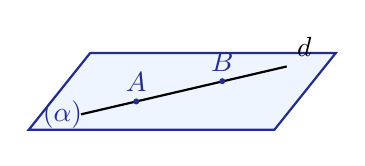
\begin{tikzpicture}[scale=.78]
\fill[lightblue] (0,0)--(4,0)--(5,1.25)--(1,1.25)--cycle;
\draw[answerblue,thick] (0,0)--(4,0)--(5,1.25)--(1,1.25)--cycle;
\draw[black,thick] (.85,.25)--(4.2,1.03) node[above right] {$d$};
\drawpoint{1.75,.46}{above}{A}
\drawpoint{3.15,.79}{above}{B}
\node[answerblue] at (.55,.25) {$(\alpha)$};
\end{tikzpicture}
\end{center}

\exampletitle{01 [TDM21]}{Cho tam giác $ABC$, điểm $M\in BC$.
Chứng minh $M\in(ABC)$, $AM\subset(ABC)$ và các mặt phẳng
$(ABC)$, $(ABM)$, $(ACM)$ trùng nhau.}
\textbf{Nhận xét từ định nghĩa:}
\[
 \left\{\begin{aligned}
  BC&\subset(ABC),\\ M&\in BC
 \end{aligned}\right.
 \Rightarrow M\in(ABC),\qquad
 \left\{\begin{aligned}
  A&\in(ABC),\\ M&\in(ABC)
 \end{aligned}\right.
 \Rightarrow AM\subset(ABC).
\]
Vì $A,B,M$ và $A,C,M$ là các bộ ba điểm không thẳng hàng
(trong tam giác không suy biến, với $M$ ở trên $BC$ và khác $B,C$),
suy ra $(ABC)=(ABM)=(ACM)$.

\propertytitle{Tính chất 5.}Nếu hai mặt phẳng phân biệt có điểm chung
thì các điểm chung của chúng tạo thành một đường thẳng. Đường thẳng
này gọi là \textbf{giao tuyến}:
\[
       d=(\alpha)\cap(\beta).
\]
\exampletitle{02 [TDM31]}{Cho hai mặt phẳng $(\alpha)$ và $(ABC)$.
Biết $AB\cap(\alpha)=M$, $AC\cap(\alpha)=N$.}
\begingroup\compactproblems
\begin{enumerate}
 \item Xác định giao tuyến của $(\alpha)$ và $(ABC)$.
 \item Nếu $BC\cap(\alpha)=P$, hãy xác định $P$.
\end{enumerate}
\endgroup

\propertytitle{Tính chất 6.}Trên mỗi mặt phẳng, các kết quả đã biết
trong hình học phẳng đều áp dụng được.

\sectitle{3}{Ba cách xác định mặt phẳng}
\begin{theorybox}
\begin{enumerate}[label=\textcolor{questionpurple}{\bfseries Cách \arabic*.},
 leftmargin=16mm,itemsep=3pt]
 \item \textbf{Ba điểm không thẳng hàng:} $A,B,C$ xác định duy nhất
 một mặt phẳng $(ABC)$.
 \item \textbf{Một đường thẳng và một điểm nằm ngoài:} $d$ và $A\notin d$
 xác định duy nhất một mặt phẳng $(d,A)$ hoặc $(A,d)$.
 \item \textbf{Hai đường thẳng cắt nhau:} $a\cap b=\{O\}$ xác định duy nhất
 một mặt phẳng $(a,b)$.
\end{enumerate}
\end{theorybox}
\begin{center}
\begin{tikzpicture}[scale=.72]
\foreach \shift in {0,4.65,9.3}{
 \begin{scope}[xshift=\shift cm]
  \fill[lightblue] (0,0)--(2.7,0)--(3.3,.92)--(.6,.92)--cycle;
  \draw[answerblue] (0,0)--(2.7,0)--(3.3,.92)--(.6,.92)--cycle;
  \node[answerblue] at (.4,.2) {$\alpha$};
 \end{scope}
}
\drawpoint{1.2,.4}{above}{A}\drawpoint{2.1,.63}{above}{B}
\drawpoint{2.1,.2}{below}{C}
\begin{scope}[xshift=4.65cm]
 \draw[thick] (.85,.32)--(2.8,.72) node[above] {$d$};
 \drawpoint{1.8,.78}{above}{A}
\end{scope}
\begin{scope}[xshift=9.3cm]
 \draw[thick] (.85,.18)--(2.7,.7) node[above] {$a$};
 \draw[thick] (1.45,.88)--(2.25,.1) node[right] {$b$};
\end{scope}
\node[below] at (1.65,-.3) {\small Ba điểm};
\node[below] at (6.3,-.3) {\small Điểm và đường};
\node[below] at (10.95,-.3) {\small Hai đường cắt nhau};
\end{tikzpicture}
\end{center}

\sectitle{4}{Hình chóp và hình tứ diện}
\textbf{\textcolor{answerblue}{4.1. Hình chóp}}

Cho đa giác lồi $A_1A_2\cdots A_n$ nằm trong mặt phẳng $(\alpha)$
và điểm $S\notin(\alpha)$. Nối $S$ với tất cả các đỉnh của đa giác,
ta được \textbf{hình chóp} $S.A_1A_2\cdots A_n$.
\begin{itemize}
 \item $S$ là \textbf{đỉnh}; đa giác $A_1A_2\cdots A_n$ là \textbf{mặt đáy}.
 \item Các tam giác $SA_1A_2,SA_2A_3,\ldots,SA_nA_1$
 là \textbf{mặt bên}.
 \item Các đoạn $SA_1,SA_2,\ldots,SA_n$ là \textbf{cạnh bên};
 các cạnh của đa giác đáy là \textbf{cạnh đáy}.
 \item Tùy theo đáy là tam giác, tứ giác, ngũ giác,\ldots\
 ta có hình chóp tam giác, hình chóp tứ giác, hình chóp ngũ giác,\ldots
\end{itemize}
\begin{center}
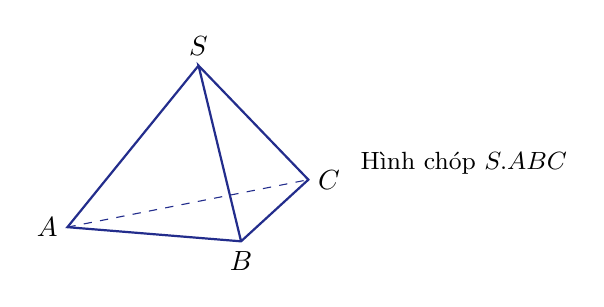
\begin{tikzpicture}[scale=.9]
 \coordinate (S) at (1.85,2.28); \coordinate (A) at (0,0);
 \coordinate (B) at (2.45,-.2); \coordinate (C) at (3.4,.67);
 \draw[answerblue,thick] (S)--(A)--(B)--(C)--(S)--(B);
 \draw[dashed,answerblue] (A)--(C);
 \node[above] at (S) {$S$};\node[left] at (A) {$A$};
 \node[below] at (B) {$B$};\node[right] at (C) {$C$};
 \node[right] at (4,.9) {\small Hình chóp $S.ABC$};
\end{tikzpicture}
\end{center}
\exampletitle{01 [TDM21]}{Xét hình chóp tam giác $S.ABC$.}
Đỉnh: $S$; mặt đáy: $(ABC)$; các mặt bên: $(SAB)$, $(SBC)$,
$(SCA)$; cạnh bên: $SA,SB,SC$; cạnh đáy: $AB,BC,CA$.

\textbf{Các công thức diện tích:}
\[
 \begin{aligned}
 S_{\mathrm{xq}}&=S_{\triangle SAB}+S_{\triangle SBC}+S_{\triangle SCA},\\
 S_{\mathrm{đ}}&=S_{\triangle ABC},\\
 S_{\mathrm{tp}}&=S_{\mathrm{xq}}+S_{\mathrm{đ}}.
 \end{aligned}
\]

\exampletitle{02 [TDM21]}{Vẽ một số hình chóp tứ giác $S.ABCD$
với các dạng đáy khác nhau.}
\begin{center}
\begin{tikzpicture}[scale=.69,line join=round]
\begin{scope}
 \coordinate (S) at (1.75,2.45);\coordinate (A) at (0,0);
 \coordinate (B) at (2.05,-.35);\coordinate (C) at (3.3,.28);
 \coordinate (D) at (.8,.95);
 \draw[answerblue,thick] (S)--(A)--(B)--(C)--(S)--(B);
 \draw[answerblue,thick] (S)--(D);
 \draw[dashed,answerblue] (A)--(D)--(C);
 \node[above] at (S) {$S$};\node[left] at (A) {$A$};
 \node[below] at (B) {$B$};\node[right] at (C) {$C$};
 \node[left] at (D) {$D$};
 \node[below,text width=3.9cm,align=center] at (1.6,-.5)
  {\small Đáy là tứ giác bất kì};
\end{scope}
\begin{scope}[xshift=5.15cm]
 \coordinate (S) at (1.8,2.45);\coordinate (A) at (0,0);
 \coordinate (B) at (3.0,0);\coordinate (C) at (2.65,.9);
 \coordinate (D) at (.65,.9);
 \draw[answerblue,thick] (S)--(A)--(B)--(C)--(S)--(B);
 \draw[answerblue,thick] (S)--(D);
 \draw[dashed,answerblue] (A)--(D)--(C);
 \node[above] at (S) {$S$};\node[left] at (A) {$A$};
 \node[below] at (B) {$B$};\node[right] at (C) {$C$};
 \node[left] at (D) {$D$};
 \node[below,text width=3.9cm,align=center] at (1.6,-.5)
  {\small Đáy là hình thang};
\end{scope}
\begin{scope}[xshift=10.15cm]
 \coordinate (S) at (1.8,2.45);\coordinate (A) at (0,0);
 \coordinate (B) at (2.3,0);\coordinate (C) at (3.05,.9);
 \coordinate (D) at (.75,.9);
 \draw[answerblue,thick] (S)--(A)--(B)--(C)--(S)--(B);
 \draw[answerblue,thick] (S)--(D);
 \draw[dashed,answerblue] (A)--(D)--(C);
 \node[above] at (S) {$S$};\node[left] at (A) {$A$};
 \node[below] at (B) {$B$};\node[right] at (C) {$C$};
 \node[left] at (D) {$D$};
 \node[below,text width=3.9cm,align=center] at (1.6,-.5)
  {\small Đáy là hình bình hành};
\end{scope}
\end{tikzpicture}
\end{center}

\textbf{\textcolor{answerblue}{4.2. Hình tứ diện}}

Cho bốn điểm $A,B,C,D$ không đồng phẳng. Hình gồm bốn tam giác
$ABC,ACD,ABD,BCD$ là \textbf{hình tứ diện $ABCD$}.
\begin{itemize}
 \item Bốn điểm $A,B,C,D$ là \textbf{đỉnh}; sáu đoạn
 $AB,AC,AD,BC,BD,CD$ là \textbf{cạnh}.
 \item Hai cạnh không có đỉnh chung là \textbf{hai cạnh đối diện}.
 Bốn tam giác $ABC,ABD,ACD,BCD$ là \textbf{bốn mặt}.
 \item Đỉnh không thuộc một mặt gọi là \textbf{đỉnh đối diện} của mặt đó.
 \item Hình tứ diện có bốn mặt đều là tam giác đều gọi là
 \textbf{tứ diện đều}; sáu cạnh của nó bằng nhau.
\end{itemize}
\begin{center}
\begin{tikzpicture}[scale=.85]
 \coordinate (A) at (1.7,2.25); \coordinate (B) at (0,0);
 \coordinate (C) at (2.25,-.2); \coordinate (D) at (3.4,.65);
 \draw[answerblue,thick] (A)--(B)--(C)--(D)--(A)--(C);
 \draw[dashed,answerblue] (B)--(D);
 \node[above] at (A) {$A$};\node[left] at (B) {$B$};
 \node[below] at (C) {$C$};\node[right] at (D) {$D$};
 \node[right] at (4.1,.8) {\small Tứ diện $ABCD$};
\end{tikzpicture}
\end{center}
Diện tích toàn phần:
\[
 \boxed{S_{\mathrm{tp}}=S_{\triangle ABC}+S_{\triangle ABD}
 +S_{\triangle ACD}+S_{\triangle BCD}.}
\]

\sectitle{5}{Cách xác định giao tuyến của hai mặt phẳng}
\begin{theorybox}
\textbf{Nguyên tắc:} Muốn tìm giao tuyến của hai mặt phẳng phân biệt
$(\alpha)$ và $(\beta)$, ta tìm \textbf{hai điểm chung phân biệt} $A,B$.
Khi đó
\[
  \boxed{A,B\in(\alpha)\cap(\beta)
  \ \Longrightarrow\ AB=(\alpha)\cap(\beta).}
\]
\textbf{Điểm chung dễ tìm:} Có thể nhận ra trực tiếp từ tên mặt phẳng,
chẳng hạn $S\in(SAB)\cap(SCD)$.

\textbf{Điểm chung khó tìm:} Dựng mặt phẳng trung gian $(\gamma)$ sao cho
\[
 a=(\alpha)\cap(\gamma),\qquad
 b=(\beta)\cap(\gamma).
\]
Nếu $a\cap b=\{M\}$ thì $M$ là điểm chung của $(\alpha)$ và $(\beta)$.
\end{theorybox}
\textbf{Mẹo tìm giao tuyến:} Khi chọn $(\gamma)$ là mặt đáy,
kéo dài các cạnh đáy (nếu cần) của hai mặt phẳng đang xét để tìm giao điểm.

\exampletitle{01 [TDM31]}{Cho hình chóp $S.ABCD$. Gọi $M,N$ lần lượt
là các điểm nằm trong tam giác $SAB$ và tam giác $SCD$.
Tìm giao tuyến của các cặp mặt phẳng:}
\begingroup\compactproblems
\begin{multicols}{2}
\begin{enumerate}
 \item $(SAB)$ và $(SAC)$.
 \item $(SAB)$ và $(SDM)$.
 \item $(SAC)$ và $(SBD)$.
 \item $(SAC)$ và $(SMN)$.
\end{enumerate}
\end{multicols}
\endgroup

\exampletitle{02 [TDM31]}{Cho tứ diện $ABCD$. Gọi $M,N,P,Q$ lần lượt
nằm trên các cạnh $AB,AC,DB,DC$; điểm $R$ nằm trong tam giác $ACD$.
Tìm giao tuyến của:}
\begingroup\compactproblems
\begin{enumerate}
 \item $(AMR)$ và $(BCD)$.
 \item $(BNQ)$ và $(CMP)$.
\end{enumerate}
\endgroup

\exampletitle{03 [TDM31]}{Cho hình chóp $S.ABC$. Các điểm $M,N$
lần lượt nằm trong các tam giác $SAB,SBC$; biết $BC$ không song song
với mặt phẳng $(AMN)$. Hãy xác định $(AMN)\cap(ABC)$.}

\sectitle{6}{Cách xác định giao điểm của đường thẳng và mặt phẳng}
Nếu hai đường thẳng $a,b$ cắt nhau tại $M$, ta viết
$a\cap b=\{M\}$ (hoặc $a\cap b=M$ theo cách viết tắt).
Tương tự, nếu đường thẳng $d$ cắt mặt phẳng $(\alpha)$ tại $M$,
ta viết $d\cap(\alpha)=\{M\}$.

\begin{theorybox}
\textbf{Bài toán:} Tìm giao điểm $M=d\cap(\alpha)$.
\begin{enumerate}[label=\textcolor{questionpurple}{\bfseries Bước \arabic*.},
 leftmargin=16mm,itemsep=3pt]
 \item Dựng một mặt phẳng trung gian $(\gamma)$ chứa $d$.
 Có thể ưu tiên mặt đáy, mặt bên hoặc mặt phẳng tạo bởi
 $d$ và một đỉnh thích hợp.
 \item Xác định giao tuyến $a=(\alpha)\cap(\gamma)$.
 \item Tìm $M=a\cap d$ (nếu hai đường thẳng cắt nhau).
 Khi đó $M\in(\alpha)$ và $M\in d$, suy ra $M=d\cap(\alpha)$.
\end{enumerate}
\[
  \boxed{d\subset(\gamma),\quad
  a=(\gamma)\cap(\alpha),\quad
  M=d\cap a\quad\Longrightarrow\quad M=d\cap(\alpha).}
\]
\end{theorybox}
\begin{center}
\begin{tikzpicture}[scale=.86]
 % mat phang alpha
 \fill[lightblue] (0,0)--(4.6,0)--(5.55,1.3)--(.95,1.3)--cycle;
 \draw[answerblue,thick] (0,0)--(4.6,0)--(5.55,1.3)--(.95,1.3)--cycle;
 % mat phang gamma
 \fill[answerblue!6] (2.0,.38)--(4.1,.38)--(4.1,3.05)--(2,3.05)--cycle;
 \draw[answerblue,dashed] (2,.38)--(4.1,.38);
 \draw[answerblue] (2,.38)--(2,3.05)--(4.1,3.05)--(4.1,.38);
 % giao tuyen
 \draw[very thick] (2,.38)--(4.1,.38) node[below right] {$a$};
 % duong d
 \draw[thick] (2.55,2.88)--(3.3,-.25) node[below] {$d$};
 \fill[questionpurple] (3.15,.38) circle (2pt) node[above right] {$M$};
 \node[answerblue] at (.63,.27) {$(\alpha)$};
 \node[answerblue] at (2.32,2.78) {$(\gamma)$};
 \node[below] at (2.85,-.62) {\small Sơ đồ hai mặt phẳng và giao điểm cần tìm};
\end{tikzpicture}
\end{center}

\exampletitle{01 [TDM31]}{Cho hình chóp $S.ABCD$ có đáy
$ABCD$ không phải hình thang.}
\begingroup\compactproblems
\begin{enumerate}
 \item Xác định $AC\cap(SBD)$ và $AB\cap(SCD)$.
 \item Gọi $M$ là trung điểm $SA$, $N$ thuộc $SB$ sao cho
 $NS=2NB$. Tìm $MN\cap(ABCD)$.
 \item Gọi $P,Q$ lần lượt là các điểm nằm trong các tam giác
 $SAB$ và $SCD$. Xác định $MQ\cap(ABCD)$ và $PQ\cap(ABCD)$.
\end{enumerate}
\endgroup

\exampletitle{02 [TDM31]}{Cho tứ diện $ABCD$. Gọi $M$ là trung điểm
$AB$, $N$ nằm trên cạnh $AC$ sao cho $NA=3NC$, $P$ nằm trên cạnh $BD$.
Xác định $CD\cap(MNP)$.}

\vspace{2mm}
\begin{tcolorbox}[colback=white,colframe=black!35,boxrule=.4pt,arc=0mm,
 left=2mm,right=2mm,top=1mm,bottom=1mm]
\footnotesize
\textbf{Nguồn nội dung:} TƯ DUY MỞ,
\emph{Vấn đề 11X31: Cơ bản về hình học không gian},
biên soạn Nguyễn Đăng Ái, trang 1--10 (PDF được cung cấp).
Đã biên tập lại dạng LaTeX, loại bỏ ô trống làm bài, quảng cáo và hình nền.
Một số đoạn chữ lặp/lạc vị trí trong bản gốc đã được chuẩn hóa;
không bổ sung lời giải cho các ví dụ chưa có lời giải trong PDF.
\end{tcolorbox}
\end{document}
